% v2-acmlarge-sample.tex, dated March 6 2012
% This is a sample file for ACM large trim journals
%
% Compilation using 'acmlarge.cls' - version 1.3, Aptara Inc.
% (c) 2011 Association for Computing Machinery (ACM)
%
% Questions/Suggestions/Feedback should be addressed to => "acmtexsupport@aptaracorp.com".
% Users can also go through the FAQs available on the journal's submission webpage.
%
% Steps to compile: latex, bibtex, latex latex
%
%\documentclass[prodmode,acmtap]{acmlarge}
\documentclass[9pt]{article}

\addtolength{\voffset}{-50pt}
\addtolength{\hoffset}{-50pt}
\addtolength{\textwidth}{100pt}
\addtolength{\textheight}{100pt}

%\usepackage[a4paper,pdftex]{geometry}
\usepackage[utf8x]{inputenc}
\usepackage[italian]{babel}
\usepackage{makeidx}
\usepackage{graphicx}

\linespread{1}

% Package to generate and customize Algorithm as per ACM style
%\usepackage[ruled]{algorithm2e}
%\SetAlFnt{\algofont}
%\SetAlCapFnt{\algofont}
%\SetAlCapNameFnt{\algofont}
%\SetAlCapHSkip{0pt}
%\IncMargin{-\parindent}
%\renewcommand{\algorithmcfname}{ALGORITHM}

% Title portion
\title{RoundWord\\
\large{Progetto per il Corso di Sistemi Distribuiti, a.a. 2012-2013}}
\author{MATTEO BRUCATO e MIRO MANNINO\\Università di Bologna}


\begin{document}

\maketitle

\begin{abstract}
% (non più di dieci righe): riassume di cosa tratta la relazione.

La presente relazione tratta della realizzazione del progetto per il corso di Sistemi Distribuiti. E' stato progettato e implementato un famoso gioco di parole, in cui i giocatori devono scrivere una parola che sia collegata alla precedente parola per mezzo di sillabe comuni (l'ultima sillaba della parola precedente e la prima sillaba della nuova parola).

Il sistema distribuito realizzato permette ad un numero arbitrario di giocatori di giocare tra loro senza l'ausilio di componenti centralizzate (eccetto il registrar per l'inizio della partita). Ciò fa sì che i guasti crash dei giocatori possano essere efficacemente individuati e gestiti, e che la partita possa continuare senza eccezioni anche nel caso in cui tutti i giocatori eccetto uno crashano.

La presente relazione descrive le tecniche utilizzate, e ne valuta i vantaggi e gli svantaggi, senza escludere le difficoltà incontrate e ciò che abbiamo imparato da questa esperienza formativa.


\end{abstract}


\tableofcontents

\newpage
\section{Introduzione}
% in cui si inquadra il problema affrontato, chiarendo gli obiettivi, riassumendo lo stato dell'arte, e descrivendo la struttura della relazione.

La presente relazione tratta della realizzazione del progetto per il corso di sistemi distribuiti, dalla sua ideazione, alle scelte progettuali, agli aspetti implementativi, non senza includere difficoltà incontrate e ciò che abbiamo imparato da questa esperienza formativa.

Un gioco molto famoso tra i bambini di ogni età, ma giocato anche tra adulti senza limiti di età, consiste nel formare sequenze di parole collegate tra di esse attraverso sillabe. Il gioco è molto semplice e non richiede nessuna strumentazione né attrezzature particolari, e può esser giocato in qualunque contesto. Per giocare, basta avere una comune conoscenza del vocabolario italiano ed essere in grado di suddividere le parole in sillabe. 

%Io direi di mettere un limite...
%Può essere giocato da un numero minimo di due giocatori, e non vi è un limite massimo.

Non essendo a conoscenza del nome del gioco (nonostante lo abbiamo giocato sin da bambini), abbiamo deciso di chiamarlo \emph{RoundWord} per il presente progetto.

%\begin{figure}
%	\begin{center}
%		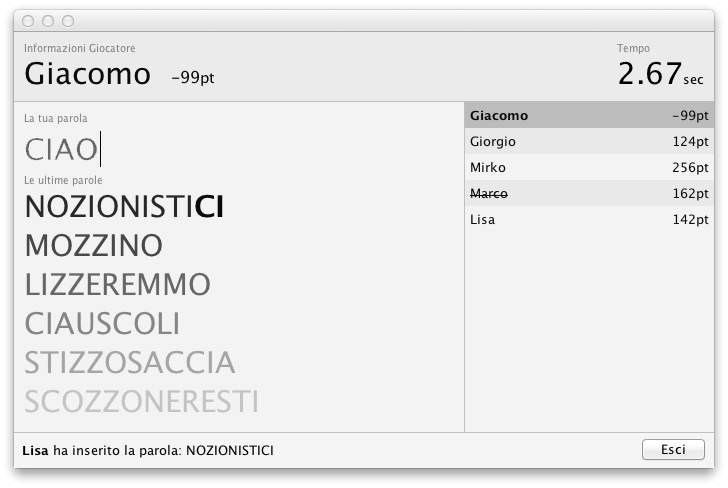
\includegraphics[scale=0.5]{imgs/screenshot.png}
%		\caption{Una screenshot del gioco dove Giacomo detiene il turno e pertanto deve inserire una parola. Notare %anche che Marco si è ritirato, oppure ha avuto un crash.}
%	\end{center}
%\end{figure}


\subsection{Regole del gioco}
All'inizio del gioco, i giocatori decidono di comune accordo una sequenza di gioco, ovvero l'ordine dei turni (giocando dal vivo, ci si mette spesso in cerchio). Ogni giocatore, al proprio turno, produrrà una singola parola. Il primo giocatore sceglie una parola qualunque, che deve essere \emph{presente nel dizionario} italiano utilizzato dal gioco. Dal secondo giocatore in poi, scatta la regola per la scelta della parola:

\begin{itemize}
\item Sia $w$ la parola prodotta dal giocatore precedente. Ad esempio ``VERIFICA''.
\item Sia $w=w_1, w_2, \dots, w_n$ la sua suddivisione in sillabe. Ad esempio, ``VE'', ``RI'', ``FI'', ``CA''.
\item Sia $w'=w'_1, w'_2, \dots, w'_m$ la parola inserita dal giocatore corrente, e la sua suddivisione in sillabe.
\item La parola $w'$ è \emph{valida} se è presente nel dizionario e se $w_n = w'_1$, ovvero se la prima sillaba della nuova parola è uguale all'ultima sillaba della parola precedente. Ad esempio, ``CARI'' e ``CARATTERISTICA'' sono tutte parole valide, mentre ``CARTA'', ``RESPIRARE'' e ``MANO'' sono tutte parole non valide.
\end{itemize}

Ciò quindi crea una sequenza di parole tutte collegate tra di esse per mezzo dell'ultima e della prima sillaba tra ogni coppia di parole. 

Per rendere più interessante il gioco, non basta che una parola sia \emph{valida} affinché si possano guadagnare dei punti per il proprio turno. Vi è un altro requisito fondamentale: la parola deve essere \emph{nuova}. Ovvero, la parola inserita non deve essere stata inserita precedentemente da alcun giocatore, durante il corso della corrente partita. Quindi, ogni giocatore deve tenere memoria della sequenza di parole generate da tutti i giocatori, ed evitare di riproporre una parola già inserita precedentemente. Per aiutare l'utente a capire le parole che sono state inserite, vengono visualizzate le ultime 6 parole.

Per complicare ulteriormente il gioco, e per evitare che il gioco duri troppo, ogni giocatore ha un limite di tempo entro il quale può proporre la sua parola.

Ogni giocatore, al proprio turno, può guadagnare o perdere punti, secondo le seguenti regole:
\begin{itemize}
\item Se la parola non è presente nel dizionario perde 80 punti.
\item Se la parola non è valida perde 80 punti.
\item Se la parola è \emph{valida}, ma non è \emph{nuova}, perde 50 punti.
\item Se il giocatore non è riuscito a produrre la parola entro il limite di tempo stabilito per un singolo turno, perde 100 punti.
\item Se la parola è valida e non è stata proposta precedentemente durante la stessa partita, il giocatore guadagna un numero di punti che dipende dalle lettere utilizzate, in base alla distribuzione delle lettere nelle parole italiane (e.g. 1 punto per la lettera A, 8 per la lettera G), dalla lunghezza della parola (i.e. 5 punti in più per ogni lettera inserita dopo la quinta), e dai millesimi di secondo impiegati (i.e. 0.02 punti per ogni millisecondo che l'utente aveva ancora a disposizione per rispondere).
\end{itemize}

Da notare che, nel caso un giocatore perda dei punti durante il proprio turno, la parola proposta non viene aggiunta alla lista delle parole utilizzate, il prossimo giocatore dovrà pertanto riprendere dalla parola dell'ultimo giocatore che era riuscito ad inserire una parola valida e nuova.

Un giocatore può ritirarsi in qualunque momento. In quel caso, il gioco continua tra i giocatori rimanenti, richiudendo il cerchio nella maniera naturale. Il gioco finisce quando un giocatore rimane da solo, oppure quando nessun giocatore riesce a produrre parole valide e nuove per un intero ciclo di gioco. Nel primo caso, il vincitore è l'unico ``superstite''. Nel secondo caso è quello con il punteggio maggiore tra i giocatori superstiti.

\subsection{Obiettivi del progetto}

L'obiettivo principale del presente progetto è la realizzazione del gioco in un ambiente distribuito, in cui varie entità distribuite (che chiameremo \emph{peer}, vista la loro intrinseca natura client/server) comunicano tra loro attraverso una rete asincrona, non affidabile, come quella di Internet. In questo tipo di contesto sono necessari coordinazione tra i peer e gestione di stati condivisi. Infatti, lo stato del gioco, composto di elementi che devono essere condivisi tra i vari peer in maniera coerente, non può risiedere in un unico peer che funge da nodo centrale.

Sono state fatte delle semplificazioni importanti per evitare alcuni degli problemi più difficili da affrontare, tutte riportate dalle specifiche del progetto. Per prima cosa si assume di avere delle comunicazioni affidabili, che i processi possono avere solamente guasti di tipo crash e che il tempo possa essere usato per catturare i peer crashati. Ciò significa che assumiamo sempre che un peer che non riusciamo a contattare per un certo periodo di tempo sia un peer che ha subito un crash, escludendo fallimenti della rete o temporanee indisponibilità del peer stesso (per lenti o crashati sono indistinguibili). 

Alcuni problemi correlati a queste assunzioni sono comunque stati risolti. Ad esempio, un peer che, precedentemente dichiarato crashato, tornasse a comunicare con i peer della rete, verrebbe comunque ignorato: il giocatore vedrà comparire un messaggio che lo avverte del fatto che è stato escludo dalla partita per connessione troppo lenta (come avviene in molti giochi commerciali).

Inoltre, secondo le specifiche, il paradigma di comunicazione utilizzato è quello di \emph{remote invocation}, in particolare il \emph{Remote Method Invocation} (RMI) di Java. Ciò fornisce un modo semplice ed ad alto livello per comunicare tra i vari peer, che ha semplificato molto l'implementazione delle comunicazioni tra di essi, in quanto tale middleware permette di mascherare l'eterogeneità tra le varie macchine. Ciononostante non è sufficiente da solo per fornire tutte le funzionalità di un ambiente distribuito, come la coordinazione, la gestione degli errori e del tempo. Tali sono quindi gli obiettivi principali del presente progetto.

\section{Aspetti progettuali}
% in cui si illustra il progetto svolto; in particolare si discutono i problemi specifici affrontati, le soluzioni valutate e proposte, e l'architettura astratta del sistema sviluppato.

\subsection{Interpretare RoundWord come un sistema distribuito}
Interpretare questo gioco nell'ambito dei sistemi distribuiti non è particolarmente difficile. Infatti, ogni giocatore è controllato da un \emph{peer}, in una rete distribuita in stile peer-to-peer (senza overlay). I turni a ciclo suggeriscono l'idea di un protocollo in stile \emph{token-ring}, dove il detentore del turno viene equiparato al \emph{leader} attuale, e la leadership viene passata al prossimo peer allo scadere di ogni turno (per questo motivo ci riferiremo a \emph{leader}, \emph{detentore del turno} o \emph{coordinatore} come sinonimi). Lo \emph{stato condiviso} tra i peer partecipanti consiste in:
\begin{itemize}
\item La lista dei peer (crashati e non crashati).
\item La lista dei punteggi dei rispettivi giocatori.
\item La lista completa delle parole inserite dai giocatori.
\item L'identità del detentore del turno attuale (ovvero del leader attuale).
\end{itemize}


\subsection{Architettura astratta}

\begin{figure}
\centering
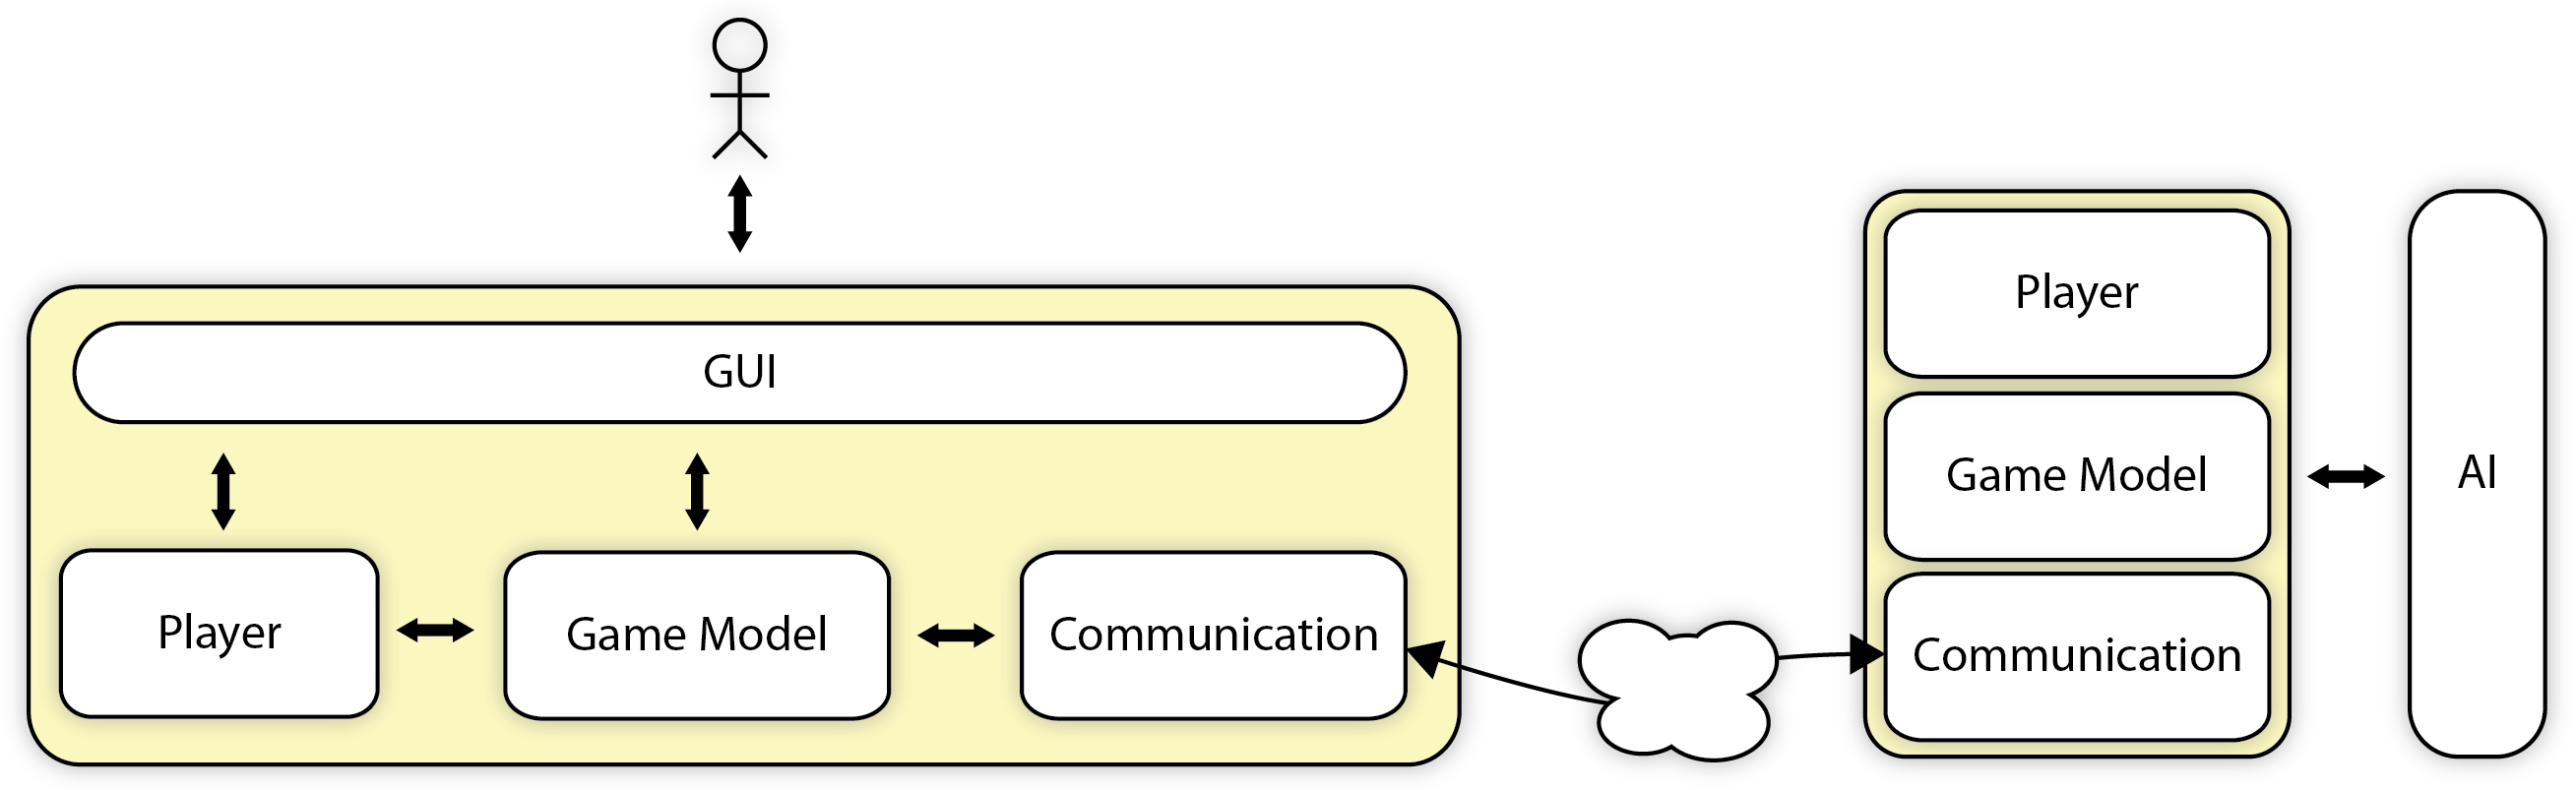
\includegraphics[scale=0.6]{imgs/ArchitetturaAstratta.png}
\caption{Architettura astratta del sistema}
\label{img:architettura-astratta}
\end{figure}

Il sistema, a livello astratto, è composto da tre componenti principali ben distinte tra loro: (1) il \emph{modello del gioco}, (2) il \emph{controllore dei giocatori} e (3) il \emph{modulo di comunicazione}. Le tre componenti sono rappresentate in Figura~\ref{img:architettura-astratta}.

La parte di modellazione del gioco comprende tutte le componenti del gioco stesso, come ad esempio il tavolo di gioco, i giocatori e la gestione delle parole del dizionario.
Questo modulo ignora il fatto che il gioco venga eseguito in rete o in locale, con utenti reali o intelligenze artificiali.
Pertanto, esso fornisce solamente dei metodi per cambiare lo stato del gioco, e genera eventi per segnalare tali cambiamenti.

Il controllore dei giocatori gestisce le azioni dei giocatori e ne riporta le scelte sul modello di gioco. Per semplicità nel debugging (e per maggior divertimento) abbiamo previsto che il gioco possa essere giocato sia da utenti reali che da intelligenze artificiali (AI). Una semplice AI è stata anche realizzata nel corso del progetto. Il controllore può essere quindi di due tipi: una GUI, per chiedere e ricevere input dall'utente e fornirgli output, e una AI, che simula le azioni di un giocatore ``reale''.
%possono essere di tre tipi: un'interfaccia grafica che comunica con il giocatore reale permettendogli di poter giocare, un peer remoto che interagisce sfruttando la parte di comunicazione, o un giocatore automatico (principalmente utilizzato per debug, ma che comunque non si esclude possa essere utilizzato come un rimpiazzo per i giocatori che hanno subito un guasto).

Il modulo di comunicazione è la parte centrale del sistema distribuito, in quanto gestisce l'interazione tra i peer del sistema. I compiti principali di questo modulo sono quelli di permettere lo scambio dei messaggi del gioco (le nuove parole inserite dai giocatori), la gestione dello stato condiviso e l'implementazione dei protocolli di gestione dei guasti di tipo crash.
%Ogni peer ha il compito di gestire un particolare giocatore, eseguendo delle azioni opportune per ogni tipo di evento generato dal gioco.
Ogni peer gestisce gli eventi generati dal giocatore locale e dai giocatori remoti, eseguendo di volta in volta le azioni opportune.

Per gestire le comunicazioni con gli altri peer, il modulo è suddiviso in due sotto-moduli: uno che funge da client (chiamato \emph{client side}) e uno che funge da server (chiamato \emph{server side}). Il client side gestisce i messaggi in uscita (non è altro che un thread fornito di una coda di messaggi), mentre il server side gestice i messaggi in entrata ed esegue tutte le azioni opportune, in base al tipo di messaggio ed ai dati in esso contenuti. 
Ad esempio, per gestire l'evento del giocatore locale che ha inserito una parola, un peer crea un messaggio specificando il peer destinatario e lo pone in uscita aggiungendolo semplicemente alla coda di messaggi in uscita del proprio client side; successivamente, tale messaggio verrà processato e inviato chiamando l'opportuna funzione del server side del peer destinatario.


\subsection{Protocolli distribuiti}
Nel seguito, descriveremo i protocolli di comunicazione e interazione distribuita facenti parte del modulo di comunicazione.

\subsubsection*{Inizializzazione della partita}

La procedura di inizializzazione della partita utilizza un server centrale ed è l'unica procedura del gioco che prevede componenti centralizzate. Tale scelta, oltre che essere prevista nelle specifiche, è un'importante semplificazione che elimina il bisogno di complicate procedure di discovery distribuite. Ma è anche un'assunzione realistica e molto usata in parecchi giochi commerciali.

Il server centrale, chiamato \textit{registrar}, è un server HTTP che provvede a raccogliere gli indirizzi IP e le porte dei vari peer che vogliono giocare, ed i nickname dei relativi giocatori. Tale server viene configurato in esecuzione per creare partite di $N$ giocatori, e quindi dà il via libera solo dopo che sono state fatte $N$ richieste proveniente da altrettanti giocatori differenti.

Al momento del raggiungimento delle $N$ richieste, il registrar manda, ad ogni giocatore, la lista degli utenti (e relativi peer) che parteciperanno alla partita. Tale lista $[p_1, p_2, .., p_N]$ è ordinata ed identica per tutti, stabilendo quindi quale sarà l'ordine con il quale avverranno i turni di gioco. Ogni lista di giocatori arriva ai vari peer in momenti differenti, e per questo motivo è necessario che tutti i peer siano a conoscenza del fatto che tutti gli altri l'abbiano già ricevuta prima di poter iniziare la partita. Se così non fosse il peer che detiene il turno, iniziando a giocare, potrebbe assumere falsamente che alcuni peer abbiano subito un guasto. Il peer che deve per primo iniziare a giocare (ha il turno), invia pertanto un messaggio di \textit{Hello}, attendendo che questo ritorni indietro. Nel caso in cui tale messaggio non dovesse ritornare (si utilizza un timeout), la partita viene annullata, per far sì che se ne possa ricreare una nuova. 



\subsubsection*{Gestione dei turni}

Il protocollo di gestione dei turni svolge molteplici funzionalità. Da un lato permette al detentore del turno attuale di inviare la parola scelta dall'utente agli altri giocatori partecipanti, da un altro permette di individuare eventuali guasti (di tipo crash) durante l'esecuzione del gioco.

\begin{figure}
\centering
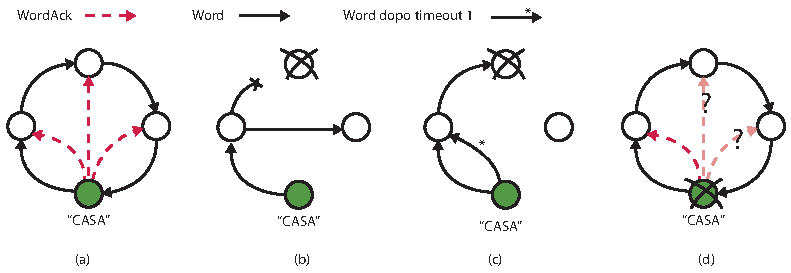
\includegraphics[scale=1]{imgs/Esempi.pdf}
\caption{Invio del messaggio Word e gestione dei guasti.}
\label{img:word}
\end{figure}

I turni ruotano in senso orario, secondo l'ordine stabilito dal registrar al momento dell'inizializzazione. Il peer corrente, denominato \emph{turnHolder}, deve inviare a tutti gli altri peer la parola scelta dal giocatore. L'invio della parola procede ad anello, attraverso un messaggio \emph{Word}, come illustrato in Figura~\ref{img:word}(a). Il turnHolder invia infatti la parola solo al peer successivo. Quest'ultimo, sapendo di non essere il turnHolder, provvederà al semplice forward della parola al peer ancora successivo, dopo aver memorizzato la parola inviatagli. Ogni turno è identificato in maniera univoca da un \emph{turnId}, fatto incrementare solo dal turnHolder al momento opportuno (creazione di una nuova parola). Ogni volta che un peer effettua un forward, però, deve attendere un ulteriore messaggio da parte del turnHolder, denominato \emph{WorkdAck}, prima di poter passare al turno di gioco successivo. Questo messaggio è necessario per catturare il guasto relativo al crash del turnHolder stesso dopo il completamento dell'anello. In Figura~\ref{img:word}(a) è evidente come il messaggio WorkAck non sia inviato anch'esso ad anello, ma sia inviato in sequenza direttamente ad ogni peer (una sorta di multicast).

Questo protocollo prevede quindi due ack. Il primo è implicitamente fornito al turnHolder dal fatto che il messaggio Word da lui inviato gli sia tornato indietro (l'ultima comunicazione che fa arrivare il messaggio al turnHolder non ha scopi informativi, solo si acknowledgement). Ciò infatti significa due cose: che l'anello è chiuso e che tutti i peer ancora attivi hanno ricevuto la nuova parola. Il secondo ack è esplicito, ed è caratterizzato dal messaggio di WordAck inviato dal turnHolder solo se il giro del messaggio Word è stato completato. Tale messaggio sancisce la fine del turno attuale e indica che anche il turnHolder ha effettuato il cambio di turno con successo.


\subsubsection*{Gestione dei guasti}
Questo protocollo è resistente a tre tipi di guasti crash: (1) il crash di un nodo della rete che non stia attivamente partecipando ad una comunicazione, (2) il crash di un forwarder del messaggio Word e (3) il crash del turnHolder. I crash vengono individuati mediante diversi timeout e relativi messaggi di acknowledgement. Essi vengono gestiti mediante ridondanza: i messaggi vengono re-inviati quando necessario. Il turnId viene utilizzato anche per ignorare messaggi relativi a turni precedenti.

\paragraph{Crash di un peer generico}
Il primo caso è raffigurato in Figura~\ref{img:word}(b). Quando un forwarder (o il turnHolder) prova a contattare un peer che è crashato, l'eccezione generata (impossibilità di connettersi al nodo) fa sì che il peer si accorga dell'errore. Quest'ultimo allora proverà semplicemente a inviare il messaggio al primo peer attivo immediatamente successivo al peer crashato. Al messaggio Word verrà incorporata l'informazione sul peer morto, in modo tale che tutti i nodi ne siano a conoscenza.

\paragraph{Crash di un forwarder}
Se invece a crashare è un forwarder, dopo aver ricevuto la parola, e prima di aver fatto il forward, quest'ultima non può essere ricevuta dal peer successivo. In tal caso, ad accorgersene, sarà il turnHolder, in quanto scatterà il primo timeout (\emph{timeout 1}). Tale timeout viene fatto partire dal turnHolder all'invio del messaggio Word, proprio per catturare il crash di nodi forwarder. Questo caso è illustrato in Figura~\ref{img:word}(c). Una volta scattato il timeout, il turnHolder invierà nuovamente il messaggio Word, con lo stesso turnId.

\paragraph{Crash del turnHolder}
Infine, potrebbe essere il turnHoder stesso a crashare. Questo è il caso più delicato, ed anche il più difficile da gestire. Infatti, il turnHolder potrebbe crashare in vari momenti: (1) prima di avere inviato il messaggio Word, oppure (2) dopo averlo inviato, prima di aver ricevuto il messaggio indietro dall'anello, e infine (3) dopo aver ricevuto indietro il messaggio Word dall'anello.

Il terzo caso è raffigurato in Figura~\ref{img:word}(d) ed è gestito attraverso un ulteriore timeout (\emph{timeout 2}) che tutti gli altri peer settano dopo aver ricevuto il messaggio Word dal turnHolder (o indirettamente, dai forwarder). I peer attendono un ulteriore acknowledgement dal turnHolder, denominato WordAck, prima di poter settare il cambio del turno. Questo ack è necessario per rispondere ai requisiti del progetto, ovvero per poter gestire almeno due guasti contemporanei di tipo crash. Se un peer non riceve tale messaggio entro il timeout, il turnHolder attuale viene considerato crashato ed è necessario stabilire chi è il detentore del turno attuale (attraverso un algoritmo simile all'elezione del leader che descriveremo successivamente).

Il secondo caso è simile al terzo, in quanto i peer che hanno ricevuto il messaggio Word faranno partire il timeout per il messaggio di WordAck, il quale scatterà e il crash del turnHolder verrà catturata e gestita allo stesso modo.

Il primo caso, invece, è il più delicato. Il turnHolder potrebbe crashare prima ancora di avere inviato il messaggio Word la prima volta. In questo caso, è necessario che gli altri peer siano in grado di identificare una morte arbitraria del turnHolder. Ciò viene fatto attraverso un ulteriore timeout, che ogni peer gestisce durante tutto il tempo del gioco. Secondo questo protocollo, il turnHolder è considerato come un leader che cede il comando ogni turno. Ogni peer si aspetta di ricevere messaggi dal leader (direttamente o indirettamente, come nel caso di un messaggio Word forwardato) entro un certo tempo. Se ciò non avviene, bisogna lanciare un algoritmo di ri-elezione del leader, per individuare chi è il prossimo turnHolder ancora attivo. Questo algoritmo è discusso nella sezione successiva.



\subsubsection*{Elezione del turnHolder}

Come detto in precedenza, vi è un'analogia tra il concetto di leader e quello di turnHolder. In particolare, il leader è il gestore attuale del turno e ha il compito di inviare a tutti la nuova parola scelta dall'utente e stabilire il cambio del turno. A differenza dei leader più comuni, che cambiano solo quando crashano, il leader del nostro gioco deve cambiare ad ogni turno in modo circolare, ovvero in senso orario ad anello. Ciò significa che, a meno di crash, è prevedibile chi sarà il prossimo leader.

Dato che ogni peer conosce gli identificativi di tutti gli altri peer, essi sanno anche chi sono i candidati leader nel momento in cui una nuova elezione deve essere eseguita. Supposto che il peer $j$ sia l'attuale leader, il peer $i$ sa che i potenziali candidati leader sono $j$, $j+1$, $\dots$, fino a $i-1$ (supponendo aritmetica modulo $N$). Se tutti loro non dovessero rispondere all'elezione, solo allora $i$ potrebbe capire di essere effettivamente lui il nuovo leader (e quindi il detentore del turno attuale). Nessun peer dopo $i$ può essere un candidato, in quanto $i$ stesso è ancora vivo.

Questo semplice ragionamento suggerisce di utilizzare l'algoritmo \emph{Bully} studiato a lezione per la realizzazione dell'elezione del leader (turnHolder) in ambiente distribuito. Infatti, in tale algoritmo si assume che tutti i peer sappiano gli identificativi di tutti gli alti peer e possano identificare univocamente i candidati leader. Quando contattato, colui che sa di essere il leader risponde con un messaggio \emph{SetTurnHolder} a tutti i peer che non sono possibili candidati, ovvero tutti i peer eccetto se stesso.

L'algoritmo Bully è tale da gestire anche i guasti eventuali durante l'elezione, a differenza dell'altro algoritmo studiato, ovvero quello ad anello. I guasti sono gestiti per mezzo di due timeout, settati entrambi da coloro che vogliono indire l'elezione, in due momenti differenti. L'algoritmo del Bully assume anche che le connessioni siano affidabili (assunzione presente nel nostro caso) e che il sistema sia sincrono, ovvero si possano usare timeout per gestire i guasti, tutte caratteristiche che lo rendono adatto al nostro contesto particolare.


\subsubsection*{Terminazione della partita}

Per la terminazione della partita è necessario che tutti i peer siano d'accordo su un unico vincitore, coerentemente con le informazioni dei punteggi di tutti i giocatori e dei peer che hanno subito un guasto. La terminazione di una partita può essere decretata da quel peer che ha proposto una parola con punteggio negativo, a seguito di un intero ciclo di turni dove ogni peer ha a sua volta ottenuto un punteggio negativo. Tale peer, essendo il detentore del turno, può quindi decidere chi sia il vincitore ed inviare tale informazione a tutti gli altri nodi, direttamente riutilizzando il messaggio di Word (per semplicità, nel messaggio Word vi è un campo extra per l'invio del vincitore), in modo che la decisione sia coerente con tutti gli altri. Questi calcola il vincitore sulla base dei punteggi dei giocatori, che i messaggi di Word hanno garantito essere uguali per tutti i nodi.

Ciò che non sappiamo con precisione istantanea sono invece le informazioni sui peer che hanno subito o stanno subendo un guasto. Per questo motivo è il turnHolder a decidere il vincitore sulla base delle informazioni che ha al momento dell'invio del messaggio di Word. Se tale messaggio, dopo avere compiuto un giro attorno all'anello, dovesse rilevare altri peer crashati, allora il turnHolder dovrebbe ricalcolare il vincitore, e se questo fosse diverso dovrebbe reinviare un nuovo messaggio di Word con il nuovo vincitore. In tal modo gestiamo il caso in cui venga decretato come vincitore un peer che abbia poi subito un guasto.

Da notare inoltre che, grazie alla gestione dei turnId nei messaggi di Word, gli ulteriori messaggi che vengono spediti vengono ignorati (ovvero non vengono aggiunte le parole nel tavolo di gioco, viene però cambiato il vincitore). Successivamente il messaggio di WordAck, che viene solitamente utilizzato per avanzare il turno, può essere visto come un \emph{commit}, che conferma definitivamente il vincitore e sancisce la fine della partita. Pertanto, alla ricezione di tale messaggio, il programma mostra a video il vincitore e termina il gioco.

\section{Aspetti implementativi}
% dettagli sulle scelte implementative, ed architettura specifica implementata. Inserire almeno il diagramma delle classi e uno delle interazioni secondo lo standard UML.

%\subsection{Architettura}

\subsection{Modellazione del gioco}

Il gioco in sé viene rappresentato da poche classi: \texttt{GameTable}, \texttt{Word}, \texttt{Player} e \texttt{Dictionary}.

La classe \texttt{Word} rappresenta una parola del gioco ed è serializzabile, per poter essere inviata via RMI. La classe \texttt{Dictionary} rappresenta un dizionario, e contiene semplici metodi per il lookup di una parola, mentre la classe \texttt{Player} rappresenta un giocatore, con un nickname, un punteggio, uno stato (attivo o non attivo).
%Consiste di una semplice stringa, ma ha numerosi metodi utili per scomporla in sillabe e determinarne il valore in punteggi. Inoltre essa è serializzabile, poiché deve poter essere inviata lungo la rete. La classe \texttt{Dictionary} rappresenta un dizionario, e contiene semplici metodi per il lookup di una parola, mentre la classe \texttt{Player} rappresenta un giocatore, con un nickname, un punteggio, uno stato (attivo o non attivo).

La classe \texttt{GameTable} rappresenta il tavolo di gioco. Essa contiene informazioni quali: la lista delle parole che sono state inserite, la lista dei giocatori, ed il giocatore che detiene il turno. Inoltre ha dei metodi per modificare lo stato del gioco, per settare il prossimo detentore del turno, o per inserire una nuova parola. Tale classe non ha un'idea del fatto di come viene controllato un giocatore; seguendo il design pattern chiamato \textit{Observer Pattern}, la classe è stata progettata per generare degli eventi, quali ad esempio l'inserimento di una nuova parola, il cambio del turno, o la terminazione del gioco. Sono poi presenti diversi listener che rispondono in maniera passiva a questi eventi seguendo delle azioni opportune, come il \texttt{Peer} che all'inserimento di una nuova parola manda dei messaggi per informare anche agli altri peer di tale evento.

\begin{figure}
	\centering
	%\vspace*{-1in}
		%\hspace*{-0.5in}
		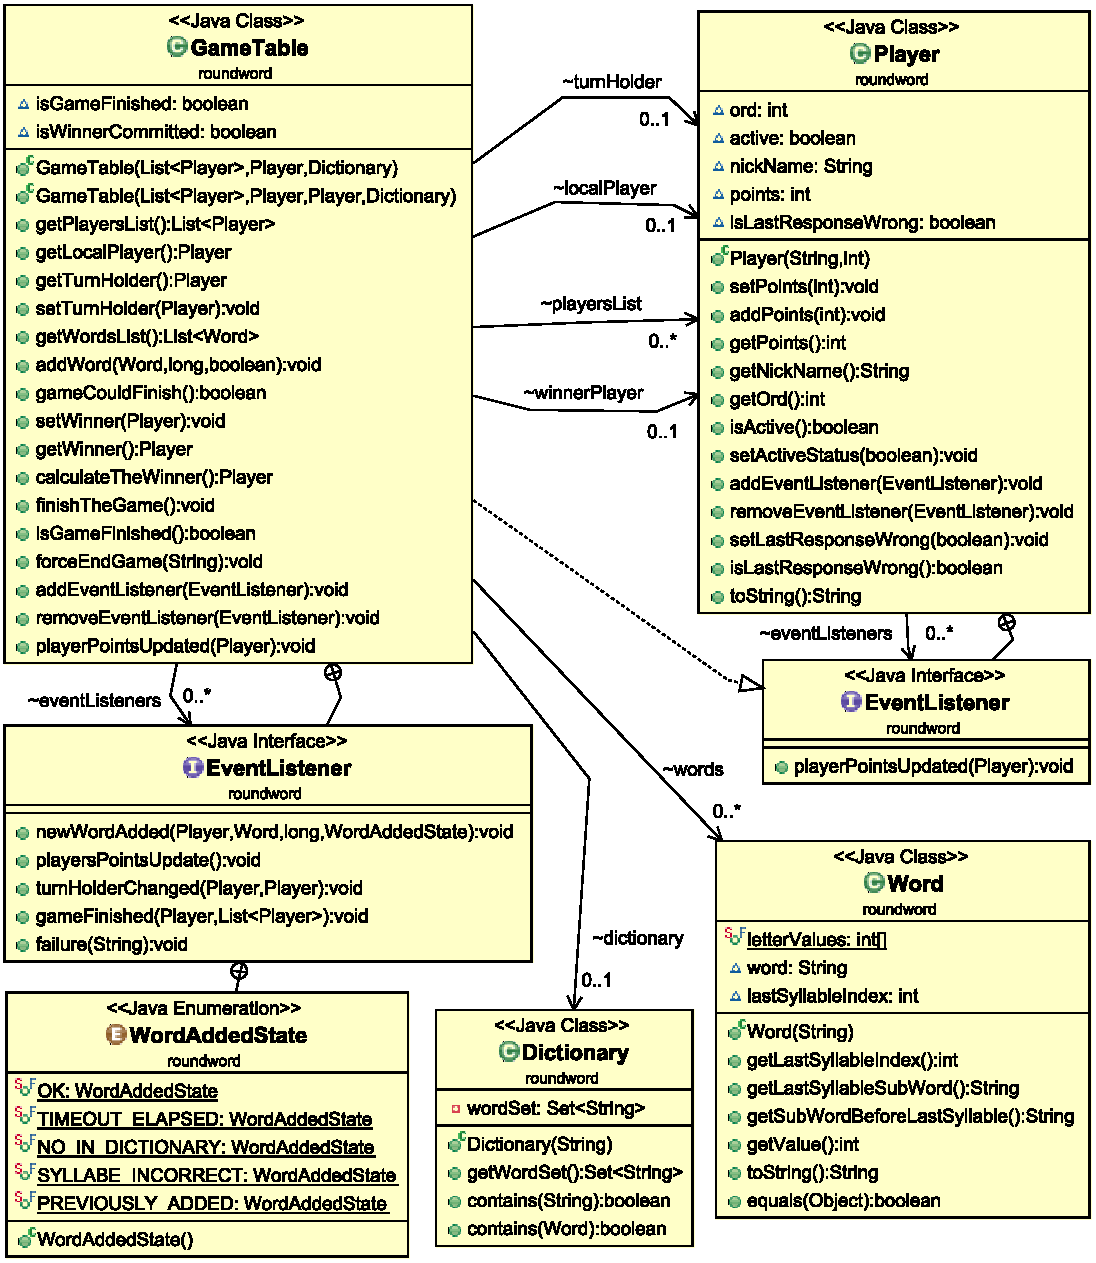
\includegraphics[scale=0.8]{imgs/ClassDiagram1.pdf}
		\caption{Il diagramma delle classi di tutta la parte di modellazione del gioco, escludendo quindi tutte le classi per far partire il gioco, le classi di comunicazione, le classi per i giocatori automatici, e le classi per l'interfaccia con l'utente.}
		\label{fig:class_diagram1}
\end{figure}

In Figura~\ref{fig:class_diagram1} possiamo osservare il diagramma delle classi di tutta la parte di modellazione del gioco. Questa, come si può intuire, comprende solamente una piccola parte dell'intera applicazione. che corrisponde agli elementi che abbiamo cercato di descrivere più nel dettaglio. Da notare che anche il \texttt{Player} può generare un evento (che avviene al cambio del punteggio), ma questi vengono esclusivamente intercettati dal \texttt{GameTable} che a sua volta genera l'evento \texttt{playerPointsUpdate()}. Quest'ultimo serve solamente alla parte dell'interfaccia per aggiornare visivamente il punteggio dei giocatori.

\subsection{Comunicazione}

\begin{figure}
	\centering
%		\hspace*{-0.2in}
		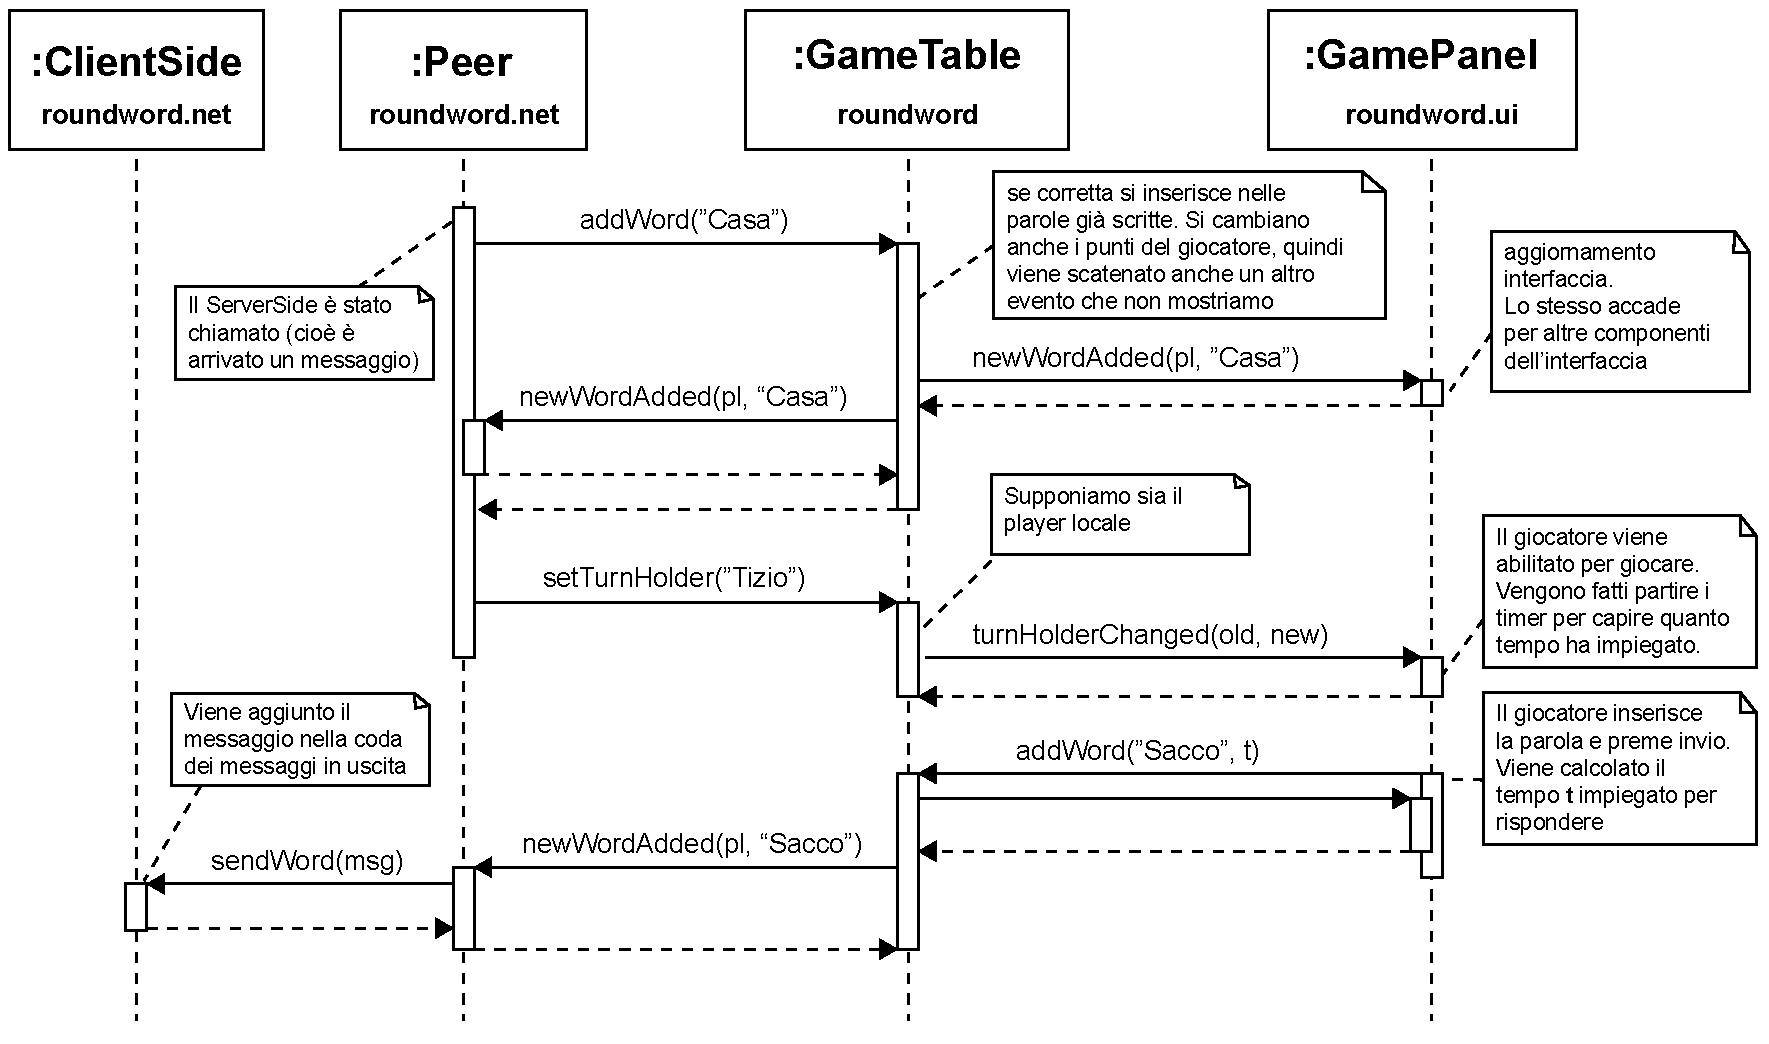
\includegraphics[scale=0.51]{imgs/Sequence1.pdf}		
		\caption{Esempio di un peer che riceve una Word da un altro peer e la comunica al GameTable. Successivamente, il WordAck fa cambiare il turno, permettendo al giocatore locale di giocare ed inserire una nuova parola. Tale parola viene inviata al peer successivo.}
		\label{fig:sequence1}
\end{figure}	


Il \texttt{Peer} è la classe che gestisce tutte le comunicazioni nella rete e gli eventi relativi. Vi un \texttt{Peer} per ogni giocatore (\texttt{Player}). Esso, al momento della creazione di un gioco, si registra come listener per intercettare gli eventi del \texttt{GameTable}. Fatto ciò, ogni volta che l'utente locale inserisce una parola, crea un messaggio di tipo \texttt{WordMsg} e lo aggiunge alla coda dei messaggi di uscita del \texttt{ClientSide} chiamando il metodo \texttt{send\_msg()}.

Il \texttt{ClientSide} è una sottoclasse di \texttt{Thread}, che nasce e muore insieme al peer, e provvede alla gestione dell'invio dei messaggi del peer. Contiene una coda di tipo \texttt{BlockingQueue} per i messaggi in uscita, senza limitazioni nella dimensione. Il metodo \texttt{send\_msg\_rmi(Msg)} altro non fa che ``eseguire'' il messaggio, raccogliendo tutti gli eventuali errori che possono essere generati da Java RMI. 
Utilizziamo il termine ``eseguire'' poiché un messaggio è in realtà un oggetto di una classe contenente un metodo \texttt{execute()}, che chiama il metodo remoto presente nel server side del peer destinatario. Ogni tipo di messaggio esegue quindi un metodo \texttt{execute()} differente, e i parametri del messaggio vengono utilizzati come argomenti per i metodi che vengono richiamati. 

Il \texttt{ServerSide} è invece una classe, istanziata solamente una volta per ogni peer, che costituisce l'insieme dei metodi che possono essere richiamati da ogni messaggio. Per esempio, il metodo \texttt{execute()} del messaggio di tipo \texttt{WordMsg} esegue il metodo del \texttt{ServerSide} del destinatario chiamato \texttt{word()}, specificando come argomenti quelli propri del messaggio: chi lo ha generato (chi detiene il turno), la parola inserita, il tempo impiegato per inserire la parola, se esiste un vincitore (cioè la partita può terminare), e la lista dei peer morti che si sono accumulati lungo il percorso.
Il seguente estratto di codice esemplifica meglio quanto appena detto e mostra le azioni intraprese dal client side per l'invio del messaggio Word via Java RMI:
\begin{verbatim}
	registry = LocateRegistry.getRegistry(destPeer.IPaddr, destPeer.serverPortno);
	stub = registry.lookup("ServerSide");
	response = stub.word(id, word, time, winnerId, crashedPeer);
\end{verbatim}

%C'è quindi un disaccoppiamento tra il peer e l'invio dei messaggi. Questo poiché, per implementare il progetto, è stato utilizzato \textit{Java RMI}, e di conseguenza inviare un messaggio equivale ad eseguire una funzione in un oggetto remoto: nel nostro caso è il client side ad eseguire la funzione nel server side del destinatario.
Da notare che il client side è stato posto su un thread separato per evitare loop di attesa infinita (si pensi all'attesa causata da un peer che non risponde, oppure a messaggi corrispondenti a chiamate ricorsive come i messaggi di Word ad anello).
%In tal modo, il peer che deve solamente fare un forward a $P_2$ del messaggio proveniente da un peer $P_1$, all'interno del metodo nel server side (invocato da $P_1$), creerà un messaggio analogo a quello generato da $P_1$, cambiando solamente il destinatario, ed incodandolo al proprio client side, con il risultato che il client side di $P_1$ termina immediatamente, senza aspettare che $P_2$ riceva il messaggio. 
Quindi, il \texttt{ClientSide} ed il \texttt{ServerSide} vengono eseguiti in thread differenti. Per questo motivo è stato molto importante gestire la concorrenza, sopratutto quando vengono modificati i campi del \texttt{Peer}. Sono stati utilizzati i meccanismi di locking messi a disposizione da Java, per garantire che nessun thread potesse compiere delle operazioni contemporaneamente sul peer. Questa decisione non è limitante in termini di efficienza, poiché la mutua esclusione è stata forzata in piccole porzioni di codice che modificano o leggono i valori del peer.

In Figura~\ref{fig:sequence1} mostriamo il diagramma di interazione tra il modulo di comunicazione e quello di modellazione del gioco. Le classi dell'interfaccia mostrate nel diagramma non sono state menzionate poiché inutili ai fini del progetto di sistemi distribuiti. Notiamo solamente che il \texttt{GamePanel} è una componente dell'interfaccia che si occupa di inserire le parole da parte dell'utente.

\begin{figure}
	\centering
%	\vspace*{-0.5in}
%		\hspace*{-0.45in}
		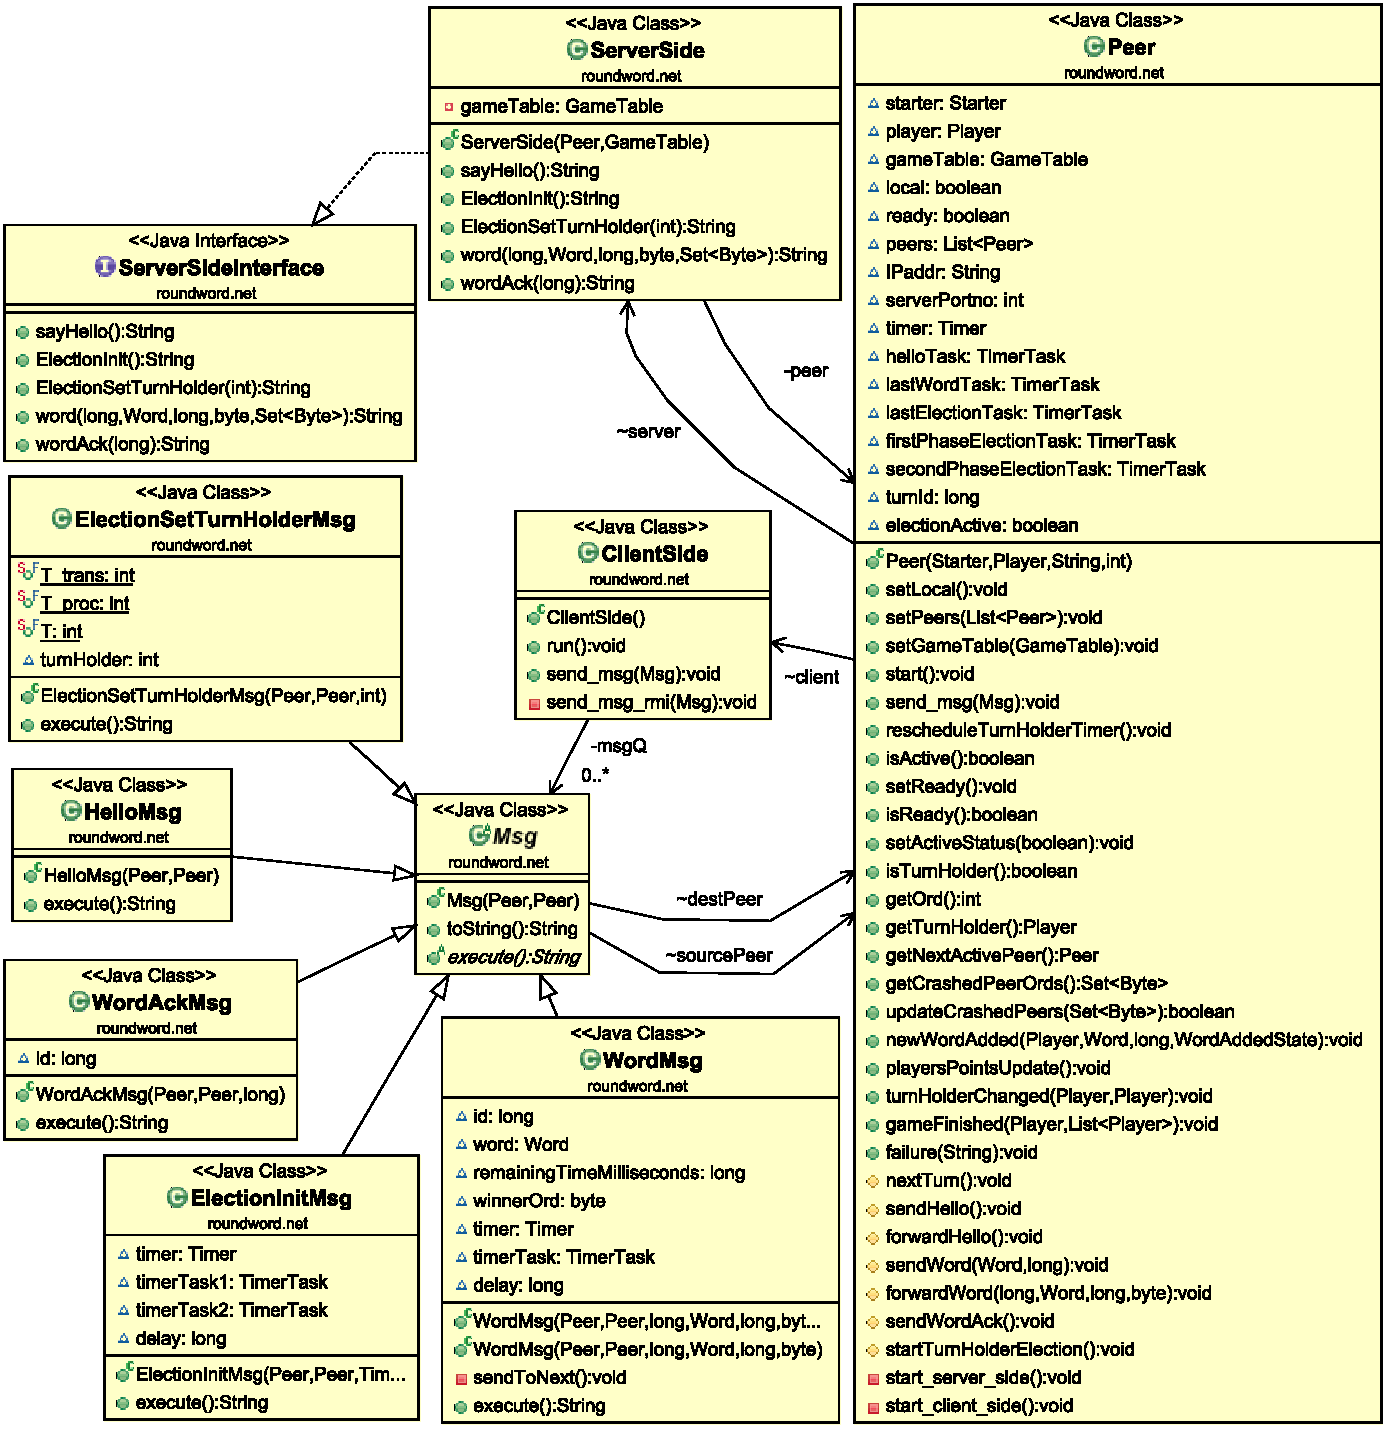
\includegraphics[scale=0.65]{imgs/ClassDiagram2.pdf}
		\caption{Il diagramma delle classi di tutta la parte di comunicazione del gioco. Da notare \texttt{ServerSideInterface} che estende la classe \texttt{Remote}, e quindi viene solamente utilizzata per Java RMI, in modo che i client side dei vari peer possano chiamare in remoto i metodi del \texttt{ServerSide}.}
		\label{fig:class_diagram2}
\end{figure}

I timeout sono stati realizzati per mezzo della classe di Java chiamata \texttt{Timer}. Un timer, memorizzato all'interno del \texttt{Peer}, si occupa di eseguire determinati \texttt{TimerTask} dopo un certo periodo di tempo (timeout). Questi task vengono annullati in seguito ad eventi opportuni, e sono quindi memorizzati anch'essi all'interno del \texttt{Peer}.
%Ogni task viene comunque memorizzato all'interno del \texttt{Peer} stesso, in modo che ogni metodo (del \texttt{Peer}, \texttt{ClientSide} o \texttt{ServerSide}) possa crearli, e salvandoli abbiamo la possibilità (anche da parte di altri metodi) di poterli annullare.
I task utilizzati sono i seguenti:
\begin{itemize}
\item \texttt{helloTask}: per catturare il fatto che il messaggio \textit{Hello} non è tornato indietro.
\item \texttt{lastWordTask}: per catturare la morte dei forwarder del messaggio \textit{Word}.
\item \texttt{lastElectionTask}: per catturare la morte del peer che detiene il turno attuale.
\item \texttt{firstPhaseElectionTask}: per catturare la morte dei peer candidati durante l'elezione.
\item \texttt{secondPhaseElectionTask}: per catturare la morte del peer eletto nella seconda fase dell'elezione.
\end{itemize}

Ognuno di questi viene creato e distrutto in momenti differenti. Ad esempio \texttt{lastWordTask} viene creato al momento dell'invio di un messaggio di \textit{Word}, e ricreato quando invece si riceve un nuovo messaggio.

\section{Valutazione}
% confronto delle soluzioni proposte con soluzioni analoghe allo stato dell'arte.

Il sistema realizzato è un gioco di parole distribuito, che per tutta la durata della partita detiene stati globali coerenti tra tutti i nodi, senza componenti centralizzate (escludendo la registrazione). Ogni partecipante è un'entità simile alle altre (\emph{peer}) e un guasto (crash) di una qualunque di esse non pregiudica il funzionamento globale del sistema. I peer possono crashare ed i crash vengono identificati e gestiti in maniera opportuna, permettendo ai partecipanti rimanenti di continuare a giocare. Una soluzione totalmente centralizzata sarebbe stata certamente molto più semplice da realizzare, ma avrebbe creato tutti i problemi tipici dei sistemi non distribuiti. In particolare, ci sarebbe stato un \emph{single point of failure}, e la presenza di possibili colli di bottiglia, rendendolo anche molto più sensibile ad attacchi di tipo DoS.

La soluzione proposta è particolarmente efficiente per quanto riguarda la dimensione dei messaggi scambiati tra i peer nella rete. Infatti, una soluzione meno efficiente che era stata inizialmente valutata prevedeva l'invio di tutto lo stato condiviso dopo ogni azione. In altre parole, il turnHolder calcolerebbe il nuovo stato e lo invierebbe per intero ad ogni peer. Ogni messaggio quindi conterrebbe tutta la lista delle parole finora prodotte, la quale cresce nel tempo. Il nostro protocollo, invece, costruisce il nuovo stato in maniera incrementale, inviando solamente gli ultimi update dello stato, e ogni peer ne calcola la nuova versione indipendentemente. In termini della dimensione dello stato, i nostri messaggi hanno dimensione O(1).

%Il gioco che è stato implementato segue le caratteristiche del classico gioco che ha avuto tanto successo, chiamato \textit{Ruzzle}, versione virtuale del noto gioco \textit{Il Paroliere}. Allo stesso modo si è pensato quale potesse essere un gioco con le stesse caratteristiche, che potesse essere anche implementato come progetto per questo corso di Sistemi Distribuiti. Tale gioco è molto citato nei libri ed in giro per il Web, ma viene pressoché giocato senza l'ausilio di un computer, o comunque senza l'ausilio di un entità completamente automatica che controlli la validità delle parole (ad esempio si utilizzano dei forum con dei moderatori umani). Questo probabilmente perché è molto difficile riuscire a costruire un algoritmo che faccia una sillabazione perfetta, per via delle tante eccezioni che sono presenti. Per questo motivo è già stato un passo avanti riuscire ad creare qualcosa di innovativo in questo senso, riuscendo a superare tali difficoltà.

Il nostro gioco è anche facilmente integrabile grazie alla sua architettura aperta ed estendibile. Il registrar è stato realizzato con HTTP (similmente a ciò che viene fatto i molti giochi commerciali), ed utilizza Java RMI per permettere di essere utilizzato in diverse architetture. Un porting su Android non sarebbe particolarmente complesso.

%TODO: Valutazioni a livello di comunicazione?

\section{Conclusioni e possibili sviluppi futuri}
% commenti conclusivi su possibili miglioramenti di quanto discusso, e possibili linee di intervento futuro.

Le sfide poste dal presente progetto sono state molteplici. Da puri problemi di tipo implementativo, come la gestione dei thread e delle parti client e server all'interno dei peer, e dell'invio dei messaggi via RMI, a problemi più tipici dei sistemi distribuiti. Il requisito di dover gestire almeno due guasti di tipo crash ci ha costretto a riflettere molto approfonditamente sul problema del numero degli acknowledgement per i nostri protocolli di cambio turno. Aver utilizzato un'architettura naturalmente ad anello ha semplificato moltissimo la gestione del primo guasto, in quanto l'acknowledgement è implicito alla chiusura dell'anello. Il multicast invece ha semplificato la gestione del secondo ack, in quanto un ulteriore giro dell'anello avrebbe complicato ulteriormente le cose.
Ancora, è stato interessante riuscire ad applicare il concetto di leader al nostro caso particolare. Con la nostra definizione di leader equivalente al detentore attuale del turno è stato possibile adattare l'algoritmo di elezione del Bully ed inserirlo in maniera efficace all'interno del nostro protocollo.

Ci riteniamo molto soddisfatti di aver realizzato questo sistema distribuito, toccando con mano i concetti teorici visti a lezione. D'altra parte è stato anche molto affascinante poter utilizzare un paradigma così potente come RMI, che permette una progettazione ed una stesura del codice molto chiara ed efficace.

Sarebbe interessante portare avanti questo progetto anche in ambiente mobile, dove sicuramente un gioco simile può avere successo. Per quanto riguarda la giocabilità, abbiamo pensato a diverse proposte e migliorie. Prima di tutto potrebbe essere più divertente creare dizionari divisi per sezioni, in modo da limitare l'inserimento delle parole solamente a quelle di una determinata categoria scelta all'inizio del gioco. Inoltre, sarebbe interessante, in seguito ad uno studio di usabilità, decidere se prevedere casi di terminazione differenti, come ad esempio la vittoria di un giocatore che realizza moltissimi punti con una sola parola. Potrebbe anche essere utile sfruttare i giocatori automatici (AI) per rimpiazzare i giocatori che hanno subito un crash.

Alcuni protocolli utilizzati per la parte di comunicazione potrebbero essere migliorati. Ad esempio si potrebbe considerare di far partire il gioco anche se l'inizializzazione fallisce dopo un certo numero di secondi, lasciando al gioco stesso il compito di dichiarare chi ha avuto un guasto e chi no. Ciò è stato tralasciato poiché le specifiche del progetto non prevedevano guasti che non fossero di tipo crash. Inoltre, il discovery dei peer crashati potrebbe essere velocizzato, attraverso un messaggio che gira continuamente nella rete. Tale approccio è comunque stato scartato poiché più difficile da gestire.



% Bibliography
\bibliographystyle{ACM-Reference-Format-Journals}
\bibliography{riferimenti}


\end{document}
% End of v2-acmlarge-sample.tex (March 2012) - Gerry Murray, ACM
